%% Cancers (MDPI) submission, prepared with the official MDPI LaTeX class.
%% Compile with the MDPI template files in ./Definitions (or drop this file and
%% bibliography.bib into the current template from https://www.mdpi.com/authors/latex).
\documentclass[cancers,article,submit,pdftex,moreauthors]{Definitions/mdpi}

\usepackage{tikz}
\usetikzlibrary{shapes.geometric,arrows.meta,positioning}
\usepackage{booktabs}
\usepackage{longtable}
\usepackage{tabularx}
\usepackage{siunitx}

% Metadata / back-matter commands added to recent MDPI templates. These
% \providecommand shims keep the file compilable against older local copies of
% the class; the current official Cancers template already defines them, in which
% case these definitions are ignored.
\providecommand{\TitleCitation}[1]{}
\providecommand{\AuthorCitation}[1]{}
\providecommand{\dataavailability}[1]{\vspace{6pt}\noindent\textbf{Data Availability Statement:} #1\par}
\providecommand{\institutionalreview}[1]{\vspace{6pt}\noindent\textbf{Institutional Review Board Statement:} #1\par}
\providecommand{\informedconsent}[1]{\vspace{6pt}\noindent\textbf{Informed Consent Statement:} #1\par}

\tikzset{
  box/.style={rectangle,draw,rounded corners,align=center,inner sep=6pt,
              text width=7.8cm,font=\small},
  ex/.style={rectangle,draw,dashed,align=left,inner sep=5pt,
             text width=4.2cm,font=\footnotesize},
  term/.style={rectangle,draw,rounded corners,align=center,inner sep=6pt,
               text width=5.8cm,font=\small,fill=black!4},
  arr/.style={-{Latex[length=2mm]}}
}

\Title{Trends in Objective Response Rate Across Phase~II and Phase~III Oncology Trials}
\TitleCitation{Trends in Objective Response Rate Across Phase II and Phase III Oncology Trials}
\Author{Alexei Vazquez $^{1,}$*}
\AuthorNames{Alexei Vazquez}
\AuthorCitation{Vazquez, A.}
\address{%
$^{1}$ \quad Nodes \& Links Ltd, Salisbury House, Station Road, Cambridge, CB1 2LA, UK}
\corres{Correspondence: alexei.vazquez@gmail.com}

\simplesumm{Early-phase (Phase~II) cancer trials are usually judged by the
objective response rate---the fraction of patients whose tumours shrink. It is
uncertain how well this early measure predicts the results of larger, confirmatory
(Phase~III) trials, and which drug combinations act better together than the sum of
their parts. Using results from \num{1646} trials reported on ClinicalTrials.gov
and spanning the pre- and post-2020 periods, we find that response rates have risen
over time, mainly in Phase~II; that most drug combinations are no better than
expected under independent action, although we identify a new set of mostly
immunotherapy-based combinations that exceed expectation; and that an early
response rate is only a weak predictor of the confirmatory response rate and of
patient survival. These findings support interpreting early response rates together
with survival and clinical context rather than on their own.}

\abstract{The objective response rate (ORR) is the dominant efficacy readout of
Phase~II oncology trials, yet its reliability as a measure of drug-combination
activity and as a predictor of confirmatory Phase~III results is debated. We
assembled \num{2994} treatment arms from \num{1646} Phase~II/III trials reporting
results on ClinicalTrials.gov, spanning the pre- and post-2020 periods, and
extracted ORR and median overall and progression-free survival (OS, PFS). Expected
combination ORR was computed under Bliss independence; Phase~II arms were matched to
confirming Phase~III arms by regimen, tumour type and line of therapy; and temporal
trends and the prediction of survival from response were tested. Mean ORR rose with
combination size and increased over time in Phase~II but not Phase~III. Of
\num{319} testable combinations, \num{33} were synergistic and \num{87}
antagonistic; every synergistic combination was new relative to two earlier surveys,
and \SI{76}{\percent} came from trials completing in 2020 or later, dominated by
immune-checkpoint and other targeted regimens. Across \num{157} matched pairs,
Phase~II ORR predicted Phase~III ORR only weakly ($R^{2}=0.15$), and ORR explained
only about a quarter of the variance in median survival. ORR should be interpreted
alongside combination context, clinical setting, and survival endpoints rather than
as a stand-alone surrogate.}

\keyword{objective response rate; Phase~II; Phase~III; drug combinations; Bliss
independence; surrogate endpoints; overall survival; progression-free survival;
ClinicalTrials.gov}

\begin{document}

\section{Introduction}
The objective response rate (ORR), the fraction of patients achieving a complete or
partial response by RECIST~\cite{eisenhauer2009}, is the primary efficacy endpoint
of most Phase~II oncology trials and underpins a large share of single-arm
accelerated approvals---even though oncology has the lowest clinical-development
success rate of any major therapeutic area~\cite{hay2014}. Two recurring
uncertainties attend its use. First, when agents are combined, the observed ORR
reflects an unknown mixture of additive and interacting effects, and a principled
baseline is required to distinguish genuine synergy or antagonism from the
arithmetic of independent activities. A pooled analysis of Phase~II trials showed
that a Bliss-independence null~\cite{bliss1939} captures the expected activity of
combinations and provides a lower bound against which interactions can be
scored~\cite{kang2013}; consistent with this, much of the benefit of approved
combinations may arise from independent drug action rather than additivity or
synergy~\cite{palmer2017}. A subsequent survey found that, although ORR increases
with combination size, most combinations do not exceed the additive expectation and
several are antagonistic---particularly those involving targeted
agents~\cite{azam2021}. Second, the extent to which a promising Phase~II ORR
translates into confirmatory Phase~III activity, and into meaningful survival
benefit, is uncertain: response is at best a weak surrogate for
survival~\cite{prentice1989,prasad2015}, yet it remains central to value frameworks
such as the ESMO Magnitude of Clinical Benefit Scale (ESMO-MCBS) and the ASCO Value
Framework~\cite{cherny2017,schnipper2016}.

Here we revisit both questions on a large cohort of trials reporting results on
ClinicalTrials.gov and spanning the pre- and post-2020 periods. We update the
combination-interaction analysis, extend it with an explicit
Phase~II$\rightarrow$Phase~III validation, and---going beyond the earlier
response-only surveys---add an analysis of overall and progression-free survival
over time and of the prediction of survival from response.

\section{Materials and Methods}

\subsection{Data Source and Extraction}
Studies were retrieved programmatically from the ClinicalTrials.gov API (v2),
restricted to interventional Phase~II or Phase~III trials with posted results (now
mandated for most applicable trials~\cite{zarin2016}), using two complementary
queries covering completion dates before and after 2020 so as to span both periods.
For each study we parsed the phase, condition (mapped to a controlled tumour
vocabulary), interventions, and the results outcome measures. Objective response
outcomes were identified by title and read either as counts of responders over the
arm denominator or as reported percentages; median overall and progression-free
survival were read from the corresponding time-to-event measures and converted to
months (survival \emph{rates} at a landmark time, reported as percentages, were
excluded, as were medians that were not reached). Interventions were attributed to
arms using the authoritative intervention--arm links, and regimen strings were
normalised to individual agents (combination splitting, removal of
salt/formulation/dose decorations, and dictionary-based agent resolution). Line of
therapy was inferred from the title and eligibility criteria. Cohort assembly is
summarised in Figure~\ref{fig:flow}: the final cohort comprised \num{2994} treatment
arms from \num{1646} trials (\num{1266} Phase~II, \num{358} Phase~III, \num{22}
Phase~II/III), contributing \num{1716} ORR, \num{1824} median-OS and \num{2099}
median-PFS values.

\begin{figure}[H]
\centering
\resizebox{\textwidth}{!}{%
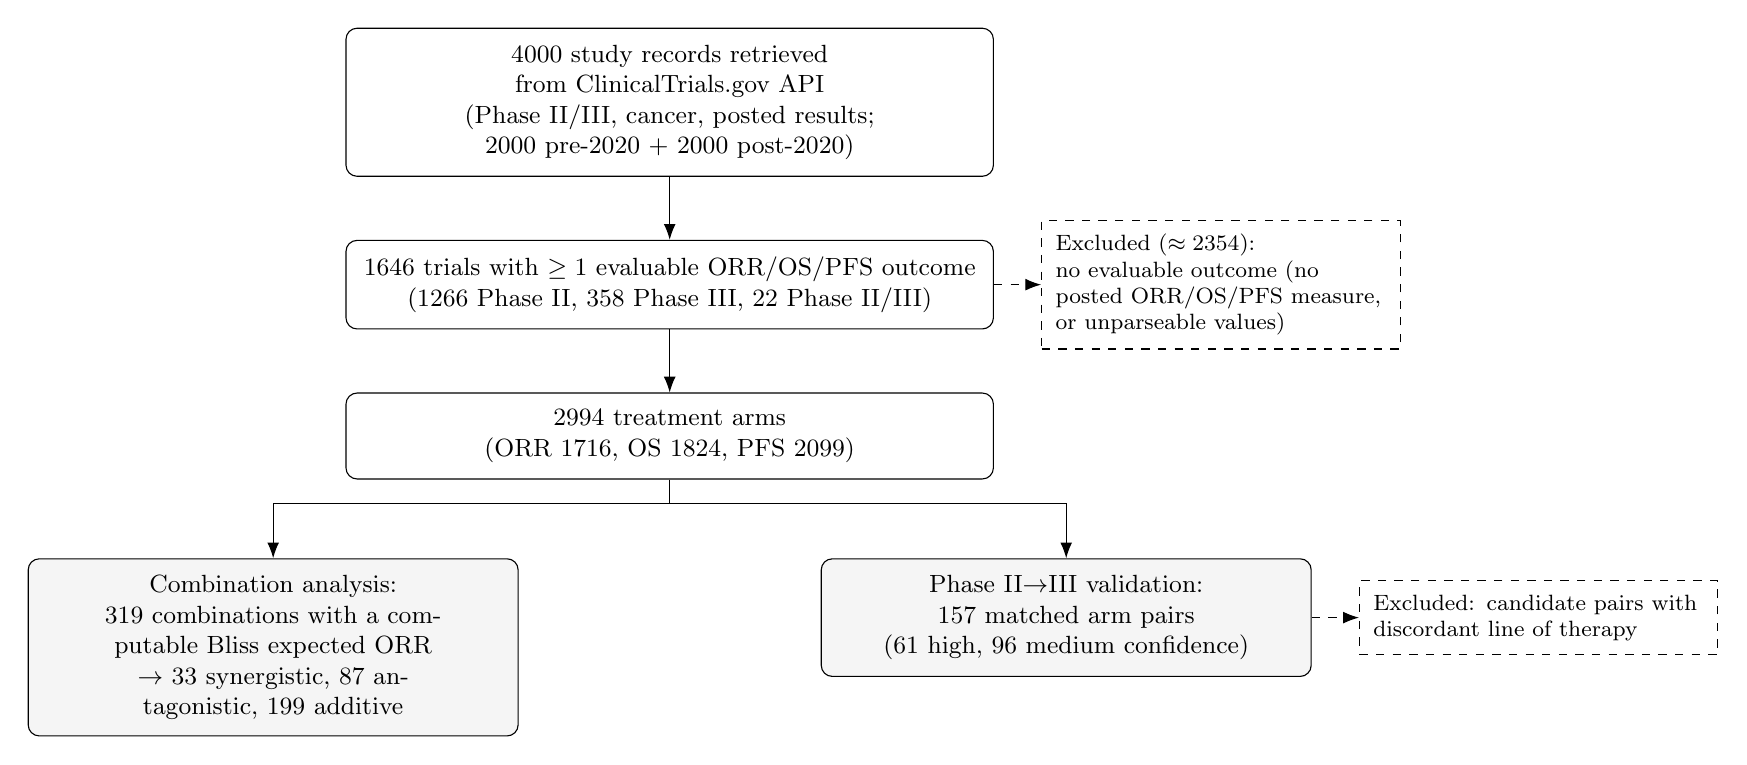
\begin{tikzpicture}[node distance=8mm]
\node[box] (a) {\num{4000} study records retrieved from ClinicalTrials.gov API\\
  (Phase~II/III, cancer, posted results; \num{2000} pre-2020 $+$ \num{2000} post-2020)};
\node[box,below=of a] (b) {\num{1646} trials with $\ge 1$ evaluable ORR/OS/PFS outcome\\
  (\num{1266} Phase~II, \num{358} Phase~III, \num{22} Phase~II/III)};
\node[box,below=of b] (c) {\num{2994} treatment arms\\
  (ORR \num{1716}, OS \num{1824}, PFS \num{2099})};
\node[term,below left=10mm and -2.2cm of c] (d) {Combination analysis:\\
  \num{319} combinations with a computable Bliss expected ORR\\
  $\rightarrow$ \num{33} synergistic, \num{87} antagonistic, \num{199} additive};
\node[term,below right=10mm and -2.2cm of c] (e) {Phase~II$\rightarrow$III validation:\\
  \num{157} matched arm pairs\\ (\num{61} high, \num{96} medium confidence)};
\node[ex,right=6mm of b] (x1) {Excluded ($\approx\num{2354}$):\\ no evaluable outcome
  (no posted ORR/OS/PFS measure, or unparseable values)};
\node[ex,right=6mm of e] (x2) {Excluded: candidate pairs with discordant line of therapy};
\draw[arr] (a)--(b); \draw[arr] (b)--(c);
\draw[arr] (c.south)--++(0,-3mm)-| (d.north);
\draw[arr] (c.south)--++(0,-3mm)-| (e.north);
\draw[arr,dashed] (b)--(x1);
\draw[arr,dashed] (e)--(x2);
\end{tikzpicture}%
}
\caption{Cohort assembly and analysis streams.\label{fig:flow}}
\end{figure}

\subsection{Expected Combination ORR and Interaction Testing}
For a combination of single agents with response probabilities $p_i$, the expected
ORR under Bliss independence is
\begin{equation}
\mathrm{ORR}_{E} \;=\; 100\%\left[\,1-\prod_i\bigl(1-p_i\bigr)\right],
\label{eq:bliss}
\end{equation}
where each $p_i$ is estimated by pooling single-agent arms of agent $i$ and taking
the mean of a Beta posterior (Jeffreys prior). The variance of $\mathrm{ORR}_{E}$
was propagated by the delta method to give a \SI{95}{\percent} interval. For each
combination arm the observed ORR was compared with $\mathrm{ORR}_{E}$ by a two-sided
exact binomial test; $p$-values were Bonferroni-corrected across all testable
combinations. A combination was called \emph{synergistic} if the observed ORR
significantly exceeded $\mathrm{ORR}_{E}$ and \emph{antagonistic} if it fell
significantly below, at a family-wise level of \SI{5}{\percent}.

\subsection{Phase~II$\rightarrow$Phase~III Validation}
Phase~II arms were matched to Phase~III arms from different trials sharing the same
regimen (set of anticancer agents), tumour type, and---where available---line of
therapy. Matches with a confirmed, identical line of therapy were labelled high
confidence; matches for which line was unknown on either side were labelled medium
confidence; matches with discordant lines were rejected. For each matched pair the
Phase~II ORR estimate (Beta posterior mean with a \SI{95}{\percent} credible
interval) was compared with the Phase~III observed ORR. Cohort agreement was
summarised by Lin's concordance correlation coefficient (CCC)~\cite{lin1989},
Pearson and Spearman correlations, $R^{2}$, the calibration slope and intercept of a
regression of the Phase~III on the Phase~II ORR (ideal slope $1$, intercept $0$),
and the Bland--Altman bias with \SI{95}{\percent} limits of
agreement~\cite{blandaltman1986}.

\subsection{Trends, Value, and Survival Analyses}
Value frameworks (ESMO-MCBS v1.1; ASCO Value Framework) grade clinical benefit from
survival, quality-of-life and toxicity data and therefore cannot be computed from
ORR alone; as a pragmatic activity proxy we applied ORR thresholds of
\SI{30}{\percent} and \SI{50}{\percent} and, for the matched pairs, assessed whether
a strong Phase~II response signal (ORR$\ge\SI{50}{\percent}$) was sustained in
Phase~III. Temporal trends in ORR, median OS and median PFS were assessed by linear
regression on trial completion year, overall and separately for Phase~II and
Phase~III. To test whether response predicts survival, arms reporting both ORR and a
median survival endpoint were analysed at the arm level: median OS (and, separately,
PFS) was regressed on ORR, with the association summarised by Pearson and Spearman
correlations and $R^{2}$.

\section{Results}

\subsection{Objective Response over Time}
Across the cohort, ORR increased modestly with trial completion year
(Figure~\ref{fig:time}). The trend was significant among Phase~II arms
($+1.1$ percentage points per year; Pearson $r=0.20$, $P<0.001$) but weak and not
significant among Phase~III arms ($+0.4$ percentage points per year; $r=0.05$,
$P=0.29$). Because the Phase~II slope was the steeper of the two, the fitted lines
converged over the study period: the Phase~III advantage in mean ORR narrowed from
about 18~percentage points in 2010 to about 7~percentage points in 2026. In the two
most recent years (2025--2026) the two phases no longer differed
significantly---mean ORR \SI{37.6}{\percent} for Phase~II ($n=168$) versus
\SI{40.1}{\percent} for Phase~III ($n=74$); Mann--Whitney $P=0.29$. This extends the
earlier survey, which reported no clear temporal trend through 2020~\cite{azam2021}:
the improvement is concentrated in early-phase testing, so that recent Phase~II
response rates have approached those seen in Phase~III. Mean ORR also increased with
the number of anticancer agents in the regimen (Table~\ref{tab:size}), from
\SI{23.8}{\percent} for single agents to \SI{45.1}{\percent} for five-drug regimens,
reproducing on a larger and more recent cohort the combination-size trend reported
previously~\cite{azam2021}; the increase was similar when restricted to regimens
containing at least one targeted agent.

\begin{figure}[H]
\centering
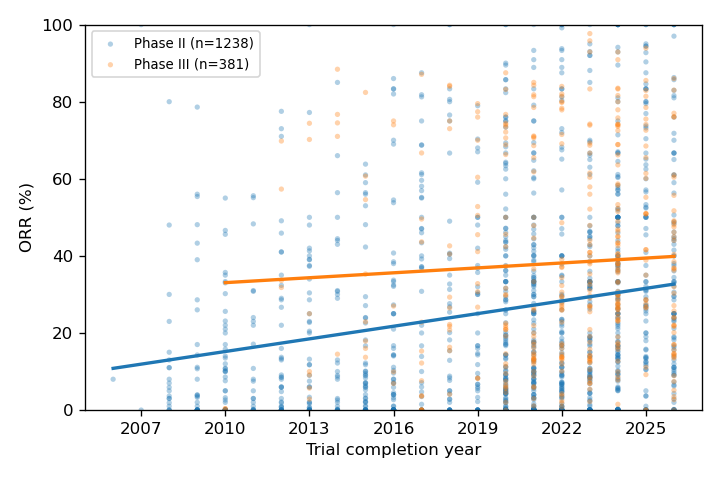
\includegraphics[width=0.72\linewidth]{figures/orr_over_time.png}
\caption{Objective response rate versus trial completion year for Phase~II and
Phase~III arms, with per-phase linear fits. Each point is a treatment arm.\label{fig:time}}
\end{figure}

\begin{table}[H]
\caption{Mean objective response rate by combination size.\label{tab:size}}
\newcolumntype{C}{>{\centering\arraybackslash}X}
\begin{tabularx}{\textwidth}{CCC}
\toprule
\textbf{Anticancer Agents} & \textbf{Arms ($n$)} & \textbf{Mean ORR} \\
\midrule
1 & 776 & \SI{23.8}{\percent} \\
2 & 606 & \SI{30.6}{\percent} \\
3 & 184 & \SI{36.9}{\percent} \\
4 &  87 & \SI{37.0}{\percent} \\
5 &  37 & \SI{45.1}{\percent} \\
\bottomrule
\end{tabularx}
\end{table}

\subsection{Synergy and Antagonism Relative to the Bliss Null}
Of \num{319} combinations with sufficient single-agent data to compute
$\mathrm{ORR}_{E}$, \num{33} (\SI{10}{\percent}) were synergistic and \num{87}
(\SI{27}{\percent}) antagonistic; the remaining \num{199} were consistent with
additivity. Antagonistic combinations thus outnumbered synergistic ones by more than
two to one, consistent with the earlier finding that combination benefit frequently
falls short of the independent-action expectation~\cite{kang2013,azam2021}.
Representative interactions are listed in Table~\ref{tab:interactions}, and the
complete set is provided in the Supplementary Tables (Table~S1, all synergistic
combinations; Table~S2, all antagonistic combinations).

Relative to the earlier surveys, which together reported \num{19} synergistic and
\num{30} antagonistic two-agent combinations from Phase~II trials through
2020~\cite{kang2013,azam2021}, our cohort identifies an order of magnitude more
significant interactions (\num{32} synergistic, \num{85} antagonistic; distinct
combinations). Almost all are newly identified---all \num{32} synergistic and
\num{78} of the \num{85} antagonistic combinations (marked with an asterisk in
Tables~S1--S2). The newly identified synergies are concentrated among recent,
targeted regimens: \num{25} of the \num{33} synergistic arms (\SI{76}{\percent})
came from trials completing in 2020 or later (median completion year 2023), \num{12}
involved an immune-checkpoint inhibitor and \num{27} at least one targeted agent. The
strongest were immunotherapy doublets and immunotherapy--targeted combinations
(tremelimumab $+$ durvalumab, cabozantinib $+$ nivolumab, ipilimumab $+$ nivolumab,
pembrolizumab $+$ lenvatinib), together with endocrine/targeted pairs such as
abiraterone $+$ enzalutamide and palbociclib $+$ fulvestrant. Among the previously
reported combinations we do recover, the antagonistic calls are largely
reproduced---nab-paclitaxel $+$ gemcitabine (confirmed across multiple independent
arms), erlotinib $+$ gemcitabine, erlotinib $+$ bevacizumab and irinotecan $+$
cetuximab all remain antagonistic---whereas some earlier synergies
(carboplatin $+$ nab-paclitaxel, rituximab $+$ ibrutinib) and one antagonism
(carboplatin $+$ gemcitabine) are consistent with additivity here, illustrating the
sensitivity of the interaction call to the pooled single-agent baselines, which
shift as trials accrue. A few 2021 combinations could not be re-evaluated, either
because the cohort contains no arm with computable single-agent baselines (e.g.,
afatinib $+$ bevacizumab, gemcitabine $+$ paclitaxel) or because composite regimen
labels were not resolved to individual agents (S-1; FOLFOXIRI).

\begin{table}[H]
\caption{Representative synergistic, additive, and antagonistic combinations.
Expected ORR is computed under Bliss independence (Equation~\eqref{eq:bliss}); the
synergistic and antagonistic combinations shown are significant after Bonferroni
correction, whereas the additive combinations are consistent with the
independent-action expectation.\label{tab:interactions}}
\newcolumntype{L}{>{\raggedright\arraybackslash}X}
\newcolumntype{C}{>{\centering\arraybackslash}X}
\begin{tabularx}{\textwidth}{lLCC}
\toprule
\textbf{Interaction} & \textbf{Combination} & \textbf{Expected ORR} & \textbf{Observed ORR} \\
\midrule
Synergy & tremelimumab $+$ durvalumab          & \SI{33}{\percent} & \SI{99}{\percent} \\
Synergy & bevacizumab $+$ paclitaxel           & \SI{30}{\percent} & \SI{88}{\percent} \\
Synergy & cabozantinib $+$ nivolumab           & \SI{29}{\percent} & \SI{56}{\percent} \\
Synergy & palbociclib $+$ fulvestrant          & \SI{15}{\percent} & \SI{44}{\percent} \\
\midrule
Additive & ipilimumab $+$ nivolumab            & \SI{31}{\percent} & \SI{30}{\percent} \\
Additive & docetaxel $+$ irinotecan            & \SI{30}{\percent} & \SI{30}{\percent} \\
Additive & pemetrexed $+$ gemcitabine          & \SI{26}{\percent} & \SI{26}{\percent} \\
\midrule
Antagonism & pemetrexed $+$ vandetanib         & \SI{72}{\percent} & \SI{8}{\percent} \\
Antagonism & buparlisib $+$ fulvestrant        & \SI{70}{\percent} & \SI{8}{\percent} \\
Antagonism & paclitaxel $+$ carboplatin        & \SI{40}{\percent} & \SI{0}{\percent} \\
Antagonism & daratumumab $+$ ixazomib $+$ lenalidomide & \SI{95}{\percent} & \SI{0}{\percent} \\
\bottomrule
\end{tabularx}
\end{table}

\subsection{Phase~II ORR Is a Weak Predictor of Phase~III ORR}
Regimen-, tumour- and line-based matching yielded \num{157} Phase~II/III arm pairs
(\num{61} high confidence, \num{96} medium confidence); candidate pairs with
discordant lines of therapy were rejected. Across all matched pairs the Phase~II ORR
was only weakly predictive of the Phase~III ORR (Table~\ref{tab:validation}):
$R^{2}=0.15$, CCC$=0.36$, with a calibration slope of $0.42$---well below the
identity---indicating pronounced regression to the mean
(Figure~\ref{fig:scatter}). The Bland--Altman bias was small ($-0.09$) but the
limits of agreement were wide ($[-0.59,\,0.42]$), so individual Phase~III outcomes
were poorly bounded by the Phase~II estimate (Figure~\ref{fig:ba}). Restricting to
line-concordant, high-confidence pairs improved agreement modestly ($R^{2}=0.19$,
CCC$=0.41$) relative to pairs with unknown line ($R^{2}=0.11$, CCC$=0.30$),
indicating that part---but not all---of the apparent unreliability of Phase~II ORR
arises from comparing trials conducted in different clinical settings. Applying
pragmatic activity thresholds, \SI{40}{\percent} of arms reached
ORR$\ge\SI{30}{\percent}$ and \SI{23}{\percent} reached ORR$\ge\SI{50}{\percent}$;
among the matched pairs, of \num{24} Phase~II arms classed as highly active
(ORR$\ge\SI{50}{\percent}$), only \num{12} (\SI{50}{\percent}) retained
ORR$\ge\SI{50}{\percent}$ in Phase~III, so roughly half of strong Phase~II response
signals were not sustained.

\begin{table}[H]
\caption{Agreement between the Phase~II ORR estimate and the Phase~III observed ORR,
overall and by match confidence.\label{tab:validation}}
\newcolumntype{C}{>{\centering\arraybackslash}X}
\begin{tabularx}{\textwidth}{lCCCC}
\toprule
\textbf{Pair Set} & \textbf{\textit{n}} & \textbf{CCC} & \textbf{$R^{2}$} & \textbf{Calibration Slope} \\
\midrule
All matched pairs                 & 157 & 0.36 & 0.15 & 0.42 \\
High confidence (line-concordant) &  61 & 0.41 & 0.19 & 0.44 \\
Medium confidence (line unknown)  &  96 & 0.30 & 0.11 & 0.37 \\
\bottomrule
\end{tabularx}
\end{table}

\begin{figure}[H]
\centering
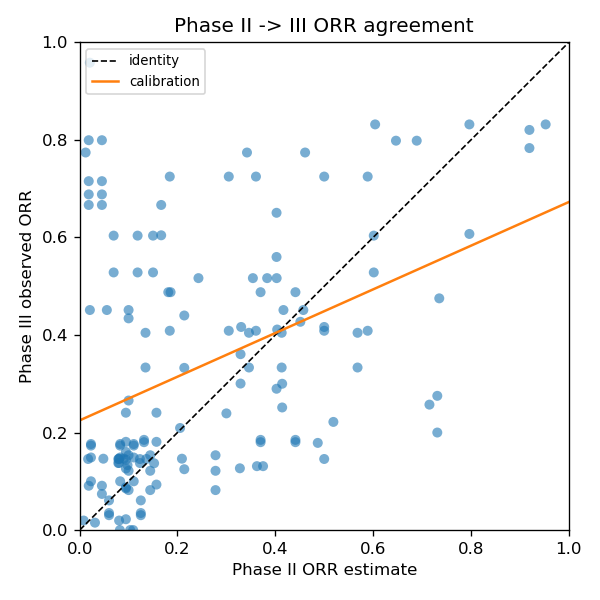
\includegraphics[width=0.62\linewidth]{figures/agreement_scatter.png}
\caption{Phase~II ORR estimate versus Phase~III observed ORR for the \num{157}
matched pairs. The dashed line is the identity; the solid line is the fitted
calibration (slope $0.42$), whose shallow slope reflects regression to the mean.\label{fig:scatter}}
\end{figure}

\begin{figure}[H]
\centering
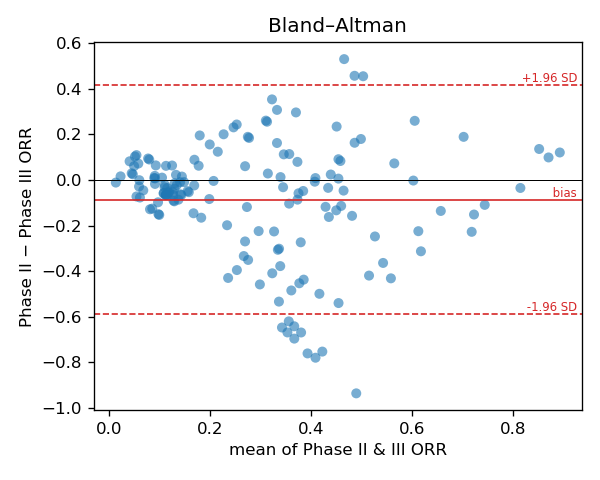
\includegraphics[width=0.62\linewidth]{figures/bland_altman.png}
\caption{Bland--Altman plot of the Phase~II$-$Phase~III ORR difference against the
pair mean. The central line is the mean bias; dashed lines are the
\SI{95}{\percent} limits of agreement.\label{fig:ba}}
\end{figure}

\subsection{Survival Trends and Prediction of Survival from Response}
Median survival was reported for a large share of arms (OS, $n=1750$; PFS,
$n=1982$). Both endpoints increased modestly over the study period
(Figure~\ref{fig:survtime}): median OS rose by about $0.36$~months per year overall
(Spearman $\rho=0.18$, $P<0.001$), most clearly in Phase~III ($0.54$~months per
year, $\rho=0.24$, $P<0.001$) and more weakly in Phase~II ($0.21$~months per year,
$P=0.002$); median PFS rose by about $0.13$~months per year overall ($P=0.002$),
again driven by Phase~III. As with ORR, the survival gains were concentrated in
later trials. At the arm level, response predicted survival: among arms reporting
both endpoints, median OS increased with ORR (Pearson $r=0.47$, $R^{2}=0.22$,
Spearman $\rho=0.47$; $n=895$) and median PFS did so somewhat more strongly
($r=0.51$, $R^{2}=0.26$, $\rho=0.62$; $n=1148$; Figure~\ref{fig:orrsurv}). Response
therefore tracks PFS a little better than OS---consistent with its position earlier
in the causal chain---but in both cases explains only about a quarter of the
variance in median survival.

\begin{figure}[H]
\centering
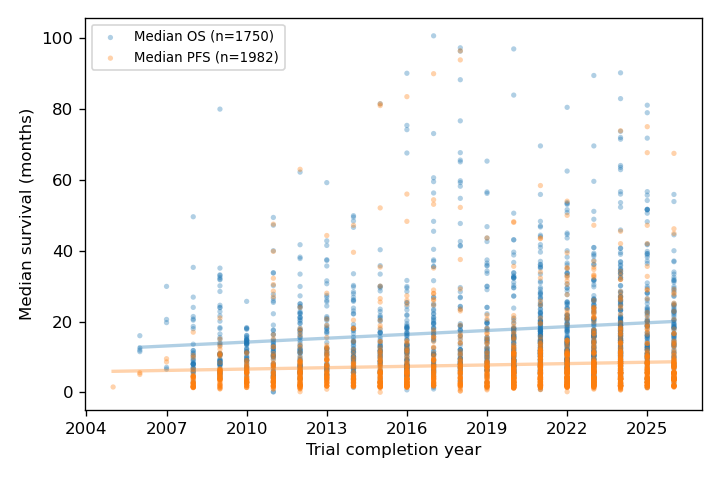
\includegraphics[width=0.72\linewidth]{figures/survival_over_time.png}
\caption{Median overall and progression-free survival (months) versus trial
completion year, with per-endpoint linear fits. Each point is a treatment arm.\label{fig:survtime}}
\end{figure}

\begin{figure}[H]
\centering
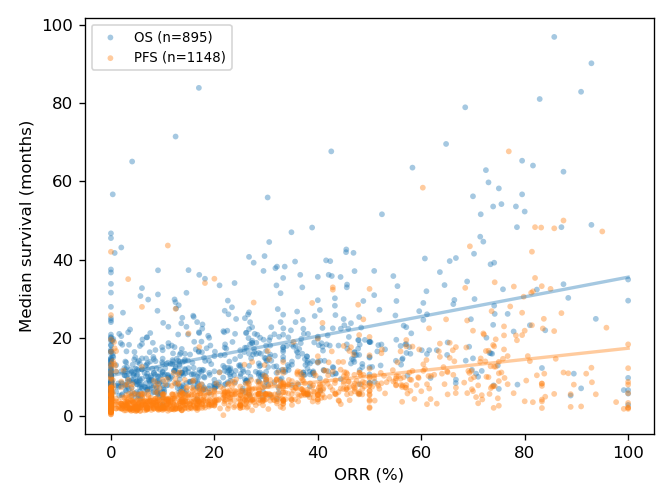
\includegraphics[width=0.62\linewidth]{figures/orr_vs_survival.png}
\caption{Arm-level median overall and progression-free survival (months) versus
objective response rate, with linear fits. Higher ORR is associated with longer
survival, more strongly for PFS than OS.\label{fig:orrsurv}}
\end{figure}

\section{Discussion}
On a large cohort spanning both the pre- and post-2020 periods we recover two
features previously described for earlier trials: ORR rises with combination size,
yet combinations are frequently non-additive, with antagonism outnumbering synergy
under a Bliss-independence null~\cite{kang2013,azam2021}; much combination benefit
may in any case reflect independent drug action rather than
synergy~\cite{palmer2017}. Unlike the earlier survey, which found no temporal
improvement through 2020~\cite{azam2021}, the extended cohort shows a modest positive
ORR trend concentrated in Phase~II. These interaction estimates are pooled across
trials and should be read as screening-level signals rather than head-to-head
comparisons.

The principal new contribution is a substantially updated catalogue of combination
interactions: every synergistic combination we identify is new relative to the two
earlier surveys, and the set is dominated by immunotherapy-based and other targeted
regimens. Why were these not seen before? The dominant reason is temporal coverage.
Three-quarters of the synergistic arms (\num{25} of \num{33}) come from trials
completing in 2020 or later---after the window of the most recent earlier survey
(through 2020) and long after the first (through $\sim$2011)---and many of the
responsible regimens (checkpoint-inhibitor doublets, cabozantinib $+$ nivolumab,
lenvatinib $+$ pembrolizumab) rely on agents approved, or first combined, only in
the last few years, so their results did not yet exist in the earlier datasets. Two
further factors contribute. First, the cohort is much larger and, unlike the
Phase~II-only predecessors, includes Phase~III arms; the pooled single-agent
response baselines are therefore better powered and more combination arms are
observed, so more combinations cross the significance threshold---this likely
accounts for the minority of pre-2020 synergies (e.g., ipilimumab $+$ nivolumab,
carfilzomib $+$ lenalidomide) that the earlier surveys did not flag. Second,
mandatory results reporting~\cite{zarin2016} has increased the fraction of
trials---especially recent ones---with structured, machine-readable outcomes on
ClinicalTrials.gov, and the automated extraction used here resolves combination and
agent names that free-text matching can miss. The new synergies are thus best read
as a genuine update of the combination landscape rather than as reinterpretations of
previously available data.

The Phase~II$\rightarrow$Phase~III analysis quantifies a long-suspected limitation: a
Phase~II ORR predicts the confirmatory Phase~III ORR only weakly ($R^{2}=0.15$),
with a calibration slope far below unity. Matching on line of therapy improves
agreement but does not eliminate the discordance, and roughly half of highly active
Phase~II arms did not sustain that activity in Phase~III. Response also correlates
with survival at the arm level but explains only about a quarter of the variance in
median OS or PFS, consistent with meta-analyses reporting generally weak associations
between response-based endpoints and survival~\cite{prasad2015,blumenthal2015}; a
strong ORR is thus likewise a weak guarantee of a survival benefit---the endpoint
that value frameworks such as ESMO-MCBS and the ASCO Value Framework actually grade.
ORR is therefore best used as an early activity filter---necessary but not
sufficient---to be complemented by survival and value-framework endpoints as
confirmatory evidence matures.

This study has limitations. The cohort is defined by the availability of posted
results on ClinicalTrials.gov and is therefore subject to reporting and selection
effects. Line of therapy is inferred heuristically from free text and is unavailable
for a subset of trials; a fraction of interventions could not be resolved to
dictionary agents and were retained as unclassified, which adds noise to
class-stratified estimates. The prediction of survival from response, and the
Phase~II$\rightarrow$Phase~III comparison, were assessed at the level of trial arms
(absolute values) rather than by formal trial-level surrogacy of treatment
effects~\cite{prentice1989,buyse2000}; matches rest on regimen, tumour and line but
not on dose, schedule, or biomarker-defined subpopulations. These estimates are
hypothesis-generating and should be confirmed with curated, trial-level surrogacy
analyses.

\section{Conclusions}
Combination ORR increases with regimen size but is frequently non-additive, and we
surface a new generation of mostly immunotherapy-based synergistic combinations not
identifiable in earlier surveys. Phase~II ORR predicts Phase~III ORR only weakly
---improving, but not resolving, when trials are matched on line of therapy---and
response explains only a minority of the variance in survival. ORR should be
interpreted jointly with combination context, clinical setting, and survival
endpoints rather than as a stand-alone surrogate.

\vspace{6pt}

\supplementary{The following supporting information can be downloaded at:
\url{https://github.com/av2atgh/oncosyn}. Table S1: all synergistic combinations;
Table S2: all antagonistic combinations (combinations new to this study are marked
with an asterisk).}

\authorcontributions{Conceptualization, A.V.; methodology, A.V.; software, A.V.;
formal analysis, A.V.; data curation, A.V.; writing---original draft preparation,
A.V.; writing---review and editing, A.V.; visualization, A.V. The author has read and
agreed to the published version of the manuscript.}

\funding{This research received no external funding. A.V. was supported by salary
from Nodes \& Links Ltd.}

\institutionalreview{Not applicable. The study used only publicly available,
de-identified, aggregate trial-level data from ClinicalTrials.gov and did not
involve human participants or animals.}

\informedconsent{Not applicable.}

\dataavailability{The trial data analysed in this study are publicly available from
ClinicalTrials.gov (\url{https://clinicaltrials.gov/}). The extraction,
normalisation, and analysis pipeline that generated these results, together with the
code to reproduce the figures and tables, is openly available at
\url{https://github.com/av2atgh/oncosyn}.}

\acknowledgments{Generative artificial intelligence (Claude, Opus~4.8; Anthropic) was
used to assist with code generation, analysis, and drafting of the text; the author
reviewed and verified all content and takes full responsibility for it.}

\conflictsofinterest{A.V. is an employee of Nodes \& Links Ltd. The company had no
role in the design of the study; in the collection, analyses, or interpretation of
data; in the writing of the manuscript; or in the decision to publish the results.}

\reftitle{References}
\externalbibliography{yes}
\bibliography{bibliography}

\clearpage
\section*{Supplementary Tables}
\setcounter{table}{0}
\renewcommand{\thetable}{S\arabic{table}}
% Auto-generated by make_supp.py -- do not edit by hand.
\begin{footnotesize}
\begin{longtable}{p{6.2cm}p{3.0cm}rrr}
\caption{All synergistic combinations ($n=32$): observed ORR significantly above the Bliss-independence expectation (Bonferroni-adjusted). Combinations marked $^{*}$ were not reported in this interaction class by Kang et al.\ (2013) or Azam \& Vazquez (2021). Exp., expected ORR; Obs., observed ORR.}\label{tab:S1}\\
\toprule
Combination & Tumour & Exp. & Obs. & Adj. $p$ \\
\midrule
\endfirsthead
\multicolumn{5}{l}{\footnotesize\itshape continued from previous page}\\
\toprule
Combination & Tumour & Exp. & Obs. & Adj. $p$ \\
\midrule
\endhead
\midrule\multicolumn{5}{r}{\footnotesize\itshape continued on next page}\\
\endfoot
\bottomrule
\endlastfoot
durvalumab + olaparib$^{*}$ & bladder & 48\% & 82\% & $<0.001$ \\
carboplatin + cisplatin + gemcitabine$^{*}$ & bladder & 34\% & 49\% & $<0.001$ \\
docetaxel + ramucirumab$^{*}$ & bladder & 16\% & 26\% & 0.016 \\
bevacizumab + paclitaxel$^{*}$ & breast & 30\% & 88\% & $<0.001$ \\
bevacizumab + capecitabine$^{*}$ & breast & 30\% & 77\% & $<0.001$ \\
fulvestrant + palbociclib$^{*}$ & breast & 15\% & 44\% & $<0.001$ \\
durvalumab + tremelimumab$^{*}$ & colorectal & 33\% & 99\% & $<0.001$ \\
lenvatinib + pembrolizumab$^{*}$ & endometrial & 26\% & 51\% & $<0.001$ \\
carboplatin + paclitaxel$^{*}$ & endometrial & 40\% & 55\% & $<0.001$ \\
bevacizumab + folfox$^{*}$ & esophageal & 17\% & 56\% & $<0.001$ \\
cisplatin + paclitaxel$^{*}$ & esophageal & 22\% & 39\% & $<0.001$ \\
carboplatin + paclitaxel + tislelizumab$^{*}$ & lung nsclc & 49\% & 74\% & $<0.001$ \\
lenvatinib + pembrolizumab$^{*}$ & lung nsclc & 26\% & 40\% & $<0.001$ \\
bevacizumab + carboplatin + irinotecan$^{*}$ & lung nsclc & 46\% & 80\% & $<0.001$ \\
durvalumab + tremelimumab$^{*}$ & lung sclc & 33\% & 100\% & 0.016 \\
bendamustine + ofatumumab$^{*}$ & lymphoma nhl & 57\% & 75\% & $<0.001$ \\
bendamustine + ofatumumab$^{*}$ & lymphoma nhl & 57\% & 73\% & 0.009 \\
lenvatinib + pembrolizumab$^{*}$ & melanoma & 26\% & 43\% & $<0.001$ \\
ipilimumab + nivolumab$^{*}$ & melanoma & 31\% & 60\% & $<0.001$ \\
ipilimumab + nivolumab$^{*}$ & melanoma & 31\% & 60\% & 0.006 \\
carfilzomib + lenalidomide$^{*}$ & myeloma & 66\% & 87\% & $<0.001$ \\
carfilzomib + lenalidomide$^{*}$ & myeloma & 66\% & 97\% & $<0.001$ \\
ixazomib + lenalidomide$^{*}$ & myeloma & 67\% & 82\% & $<0.001$ \\
ixazomib + lenalidomide$^{*}$ & myeloma & 67\% & 78\% & 0.002 \\
ixazomib + lenalidomide$^{*}$ & myeloma & 67\% & 93\% & 0.005 \\
cisplatin + nivolumab$^{*}$ & other & 19\% & 100\% & $<0.001$ \\
cisplatin + gemcitabine$^{*}$ & other & 13\% & 29\% & $<0.001$ \\
carboplatin + paclitaxel$^{*}$ & ovarian & 40\% & 93\% & $<0.001$ \\
bevacizumab + carboplatin + paclitaxel$^{*}$ & ovarian & 47\% & 96\% & $<0.001$ \\
abiraterone + enzalutamide$^{*}$ & prostate & 45\% & 98\% & $<0.001$ \\
cabozantinib + nivolumab$^{*}$ & renal & 29\% & 56\% & $<0.001$ \\
ipilimumab + nivolumab$^{*}$ & renal & 31\% & 42\% & 0.002 \\
\end{longtable}
\end{footnotesize}

\clearpage
\begin{footnotesize}
\begin{longtable}{p{6.2cm}p{3.0cm}rrr}
\caption{All antagonistic combinations ($n=85$): observed ORR significantly below the Bliss-independence expectation (Bonferroni-adjusted). Combinations marked $^{*}$ were not reported in this interaction class by Kang et al.\ (2013) or Azam \& Vazquez (2021). Exp., expected ORR; Obs., observed ORR.}\label{tab:S2}\\
\toprule
Combination & Tumour & Exp. & Obs. & Adj. $p$ \\
\midrule
\endfirsthead
\multicolumn{5}{l}{\footnotesize\itshape continued from previous page}\\
\toprule
Combination & Tumour & Exp. & Obs. & Adj. $p$ \\
\midrule
\endhead
\midrule\multicolumn{5}{r}{\footnotesize\itshape continued on next page}\\
\endfoot
\bottomrule
\endlastfoot
buparlisib + fulvestrant$^{*}$ & breast & 70\% & 8\% & $<0.001$ \\
buparlisib + fulvestrant$^{*}$ & breast & 70\% & 3\% & $<0.001$ \\
abemaciclib + trastuzumab$^{*}$ & breast & 85\% & 14\% & $<0.001$ \\
buparlisib + paclitaxel$^{*}$ & breast & 72\% & 23\% & $<0.001$ \\
buparlisib + paclitaxel$^{*}$ & breast & 72\% & 27\% & $<0.001$ \\
capecitabine + nab-paclitaxel + paclitaxel$^{*}$ & breast & 70\% & 40\% & $<0.001$ \\
abemaciclib + fulvestrant + trastuzumab$^{*}$ & breast & 87\% & 33\% & $<0.001$ \\
paclitaxel + trastuzumab$^{*}$ & breast & 87\% & 44\% & $<0.001$ \\
paclitaxel + trastuzumab$^{*}$ & breast & 87\% & 50\% & $<0.001$ \\
lapatinib + trastuzumab$^{*}$ & breast & 84\% & 22\% & $<0.001$ \\
oxaliplatin + trastuzumab$^{*}$ & breast & 90\% & 20\% & $<0.001$ \\
carboplatin + cetuximab$^{*}$ & breast & 49\% & 8\% & $<0.001$ \\
carboplatin + cetuximab$^{*}$ & breast & 49\% & 6\% & $<0.001$ \\
letrozole + palbociclib$^{*}$ & breast & 67\% & 46\% & $<0.001$ \\
palbociclib + trastuzumab$^{*}$ & breast & 84\% & 0\% & $<0.001$ \\
lapatinib + trastuzumab$^{*}$ & breast & 84\% & 50\% & $<0.001$ \\
avelumab + fulvestrant + palbociclib$^{*}$ & breast & 43\% & 13\% & $<0.001$ \\
carboplatin + cetuximab$^{*}$ & breast & 49\% & 8\% & 0.007 \\
bevacizumab + gemcitabine$^{*}$ & breast & 22\% & 0\% & 0.015 \\
atezolizumab + carboplatin$^{*}$ & breast & 35\% & 9\% & 0.021 \\
cetuximab + irinotecan + ramucirumab$^{*}$ & colorectal & 47\% & 0\% & $<0.001$ \\
cetuximab + irinotecan & colorectal & 46\% & 0\% & $<0.001$ \\
atezolizumab + bevacizumab + capecitabine$^{*}$ & colorectal & 40\% & 9\% & $<0.001$ \\
bevacizumab + capecitabine$^{*}$ & colorectal & 30\% & 4\% & 0.010 \\
china cohort - soc + durvalumab + olaparib$^{*}$ & endometrial & 79\% & 45\% & 0.009 \\
durvalumab + global cohort - soc + olaparib$^{*}$ & endometrial & 77\% & 64\% & 0.025 \\
nab-paclitaxel + ramucirumab$^{*}$ & esophageal & 53\% & 20\% & $<0.001$ \\
capecitabine + cetuximab + oxaliplatin$^{*}$ & gastric & 66\% & 23\% & $<0.001$ \\
capecitabine + docetaxel + oxaliplatin$^{*}$ & gastric & 56\% & 26\% & $<0.001$ \\
docetaxel + oxaliplatin$^{*}$ & gastric & 45\% & 23\% & 0.028 \\
bevacizumab + pembrolizumab$^{*}$ & glioma & 30\% & 0\% & $<0.001$ \\
buparlisib + paclitaxel$^{*}$ & head neck & 72\% & 14\% & $<0.001$ \\
buparlisib + paclitaxel$^{*}$ & head neck & 72\% & 39\% & $<0.001$ \\
carboplatin + cetuximab + cisplatin + docetaxel$^{*}$ & head neck & 57\% & 8\% & $<0.001$ \\
cisplatin + erlotinib + gemcitabine$^{*}$ & hepatocellular & 63\% & 7\% & $<0.001$ \\
durvalumab + tremelimumab$^{*}$ & hepatocellular & 33\% & 20\% & $<0.001$ \\
durvalumab + tremelimumab$^{*}$ & hepatocellular & 33\% & 17\% & 0.003 \\
pemetrexed + vandetanib$^{*}$ & lung nsclc & 72\% & 8\% & $<0.001$ \\
carboplatin + paclitaxel$^{*}$ & lung nsclc & 40\% & 0\% & $<0.001$ \\
carboplatin + cisplatin + ipilimumab + nivolumab + paclitaxel + pemetrexed$^{*}$ & lung nsclc & 66\% & 38\% & $<0.001$ \\
carboplatin + cisplatin + paclitaxel + pemetrexed$^{*}$ & lung nsclc & 50\% & 25\% & $<0.001$ \\
carboplatin + paclitaxel + pembrolizumab + pemetrexed$^{*}$ & lung nsclc & 60\% & 0\% & $<0.001$ \\
erlotinib + pemetrexed$^{*}$ & lung nsclc & 64\% & 17\% & $<0.001$ \\
carboplatin + cisplatin + nab-paclitaxel + paclitaxel + pemetrexed + tislelizumab$^{*}$ & lung nsclc & 79\% & 48\% & $<0.001$ \\
efatutazone + erlotinib$^{*}$ & lung nsclc & 75\% & 20\% & $<0.001$ \\
carboplatin + paclitaxel + pemetrexed$^{*}$ & lung nsclc & 50\% & 0\% & $<0.001$ \\
carboplatin + nab-paclitaxel + paclitaxel + pembrolizumab$^{*}$ & lung nsclc & 77\% & 58\% & $<0.001$ \\
carboplatin + cisplatin + pembrolizumab + pemetrexed$^{*}$ & lung nsclc & 50\% & 29\% & $<0.001$ \\
erlotinib + sorafenib$^{*}$ & lung nsclc & 61\% & 0\% & $<0.001$ \\
bortezomib + docetaxel$^{*}$ & lung nsclc & 57\% & 10\% & $<0.001$ \\
bortezomib + docetaxel$^{*}$ & lung nsclc & 57\% & 10\% & $<0.001$ \\
ipilimumab + nivolumab$^{*}$ & lung nsclc & 31\% & 15\% & $<0.001$ \\
docetaxel + pemetrexed$^{*}$ & lung nsclc & 27\% & 7\% & $<0.001$ \\
gemcitabine + nab-paclitaxel & lung nsclc & 57\% & 14\% & $<0.001$ \\
cetuximab + docetaxel + gemcitabine$^{*}$ & lung nsclc & 49\% & 17\% & $<0.001$ \\
ipilimumab + nivolumab + paclitaxel$^{*}$ & lung nsclc & 46\% & 11\% & $<0.001$ \\
carboplatin + cisplatin + nivolumab + pemetrexed$^{*}$ & lung nsclc & 48\% & 31\% & 0.008 \\
erlotinib + gemcitabine & lung nsclc & 62\% & 16\% & 0.014 \\
carboplatin + topotecan$^{*}$ & lung nsclc & 40\% & 9\% & 0.040 \\
nivolumab + rucaparib$^{*}$ & lung sclc & 49\% & 12\% & 0.004 \\
brentuximab vedotin + ibrutinib$^{*}$ & lymphoma hodgkin & 91\% & 67\% & 0.020 \\
bortezomib + rituximab & lymphoma nhl & 76\% & 28\% & $<0.001$ \\
gemcitabine + oxaliplatin + rituximab$^{*}$ & lymphoma nhl & 73\% & 44\% & 0.002 \\
daratumumab + ixazomib + lenalidomide$^{*}$ & myeloma & 95\% & 0\% & $<0.001$ \\
bortezomib + lenalidomide$^{*}$ & myeloma & 82\% & 0\% & $<0.001$ \\
bortezomib + lenalidomide$^{*}$ & myeloma & 82\% & 20\% & $<0.001$ \\
daratumumab + pomalidomide$^{*}$ & myeloma & 89\% & 69\% & $<0.001$ \\
erlotinib + everolimus$^{*}$ & neuroendocrine & 60\% & 0\% & $<0.001$ \\
cisplatin + gemcitabine + nab-paclitaxel$^{*}$ & other & 58\% & 9\% & $<0.001$ \\
ibrutinib + venetoclax$^{*}$ & other & 91\% & 7\% & $<0.001$ \\
avelumab + axitinib$^{*}$ & other & 61\% & 18\% & 0.002 \\
everolimus + letrozole$^{*}$ & other & 68\% & 37\% & 0.016 \\
bevacizumab + carboplatin + erlotinib + paclitaxel$^{*}$ & ovarian & 77\% & 0\% & $<0.001$ \\
bevacizumab + carboplatin + paclitaxel$^{*}$ & ovarian & 47\% & 0\% & $<0.001$ \\
cediranib + durvalumab + olaparib$^{*}$ & ovarian & 49\% & 0\% & $<0.001$ \\
nemvaleukin + pembrolizumab$^{*}$ & ovarian & 21\% & 9\% & 0.006 \\
cediranib + olaparib$^{*}$ & ovarian & 31\% & 3\% & 0.012 \\
cetuximab + irinotecan + oxaliplatin$^{*}$ & pancreatic & 65\% & 7\% & $<0.001$ \\
gemcitabine + nab-paclitaxel & pancreatic & 57\% & 30\% & $<0.001$ \\
gemcitabine + nab-paclitaxel & pancreatic & 57\% & 36\% & $<0.001$ \\
capecitabine + gemcitabine + nab-paclitaxel$^{*}$ & pancreatic & 66\% & 39\% & $<0.001$ \\
dostarlimab + niraparib$^{*}$ & pancreatic & 60\% & 0\% & $<0.001$ \\
gemcitabine + nab-paclitaxel & pancreatic & 57\% & 33\% & $<0.001$ \\
ipilimumab + nivolumab + sunitinib$^{*}$ & renal & 44\% & 27\% & $<0.001$ \\
bortezomib + sorafenib$^{*}$ & renal & 54\% & 6\% & 0.021 \\
\end{longtable}
\end{footnotesize}


\end{document}
